\documentclass{article}
\usepackage{graphicx}
\usepackage[margin=1.5cm]{geometry}
\usepackage{amsmath}

\begin{document}

\title{Thursday Reading Assessment: Unit 8, Momentum}
\author{Prof. Jordan C. Hanson}

\maketitle

\section{Memory Bank}

\begin{itemize}
\item $P_1 V_1 / T_1 = P_2 V_2 / T_2$ ... Collection of ideal gas scaling relationships.
\end{itemize}

\section{Momentum}

\begin{enumerate}
\item
\begin{figure}[ht]
\centering
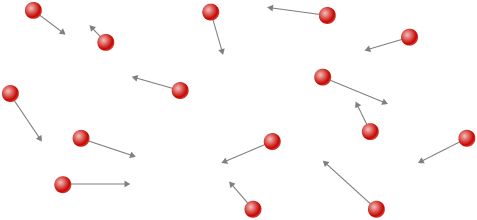
\includegraphics[width=0.35\textwidth]{gas1.jpeg}
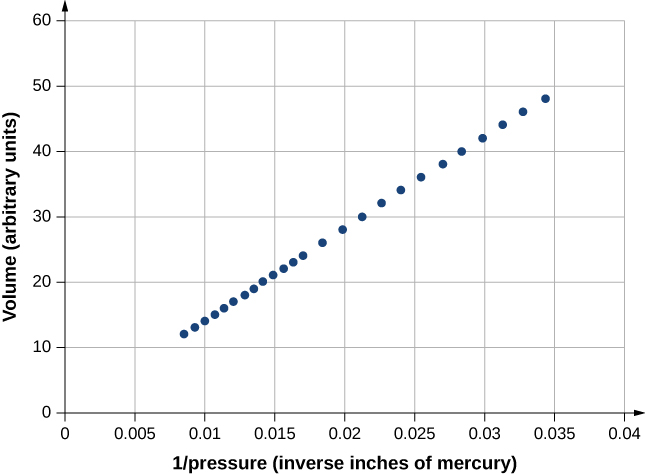
\includegraphics[width=0.45\textwidth]{gas2.jpeg}
\caption{\label{fig:collision} (Left) Molecule model of an ideal gas. (Right) Data demonstrating one of the scaling relationships.}
\end{figure}
Suppose a gas has a pressure of 10 kilo-pascals and is inside a piston with a volume of 1 liter.  If the temperature is held constant, and the volume is compressed to 0.5 liters, what is the new pressure? \\ \vspace{3cm}
\item Suppose a gas has a pressure of 10 kilo-pascals and is inside a piston with a volume of 1 liter.  If the volume is held constant, and the temperature is increased from 300 degrees Kelvin to 600 degrees Kelvin, what is the new pressure? \\ \vspace{2cm}
\end{enumerate}
\end{document}
